\chapter[Metodologia]{Metodologia}


Este capítulo foi elaborado para melhorar o entendimento das atividades
 realizadas para a produção deste trabalho. O fluxo da Figura 
\ref{fig:fases_metodologia} define estas atividades.

\begin{figure}[h]
    \centering
        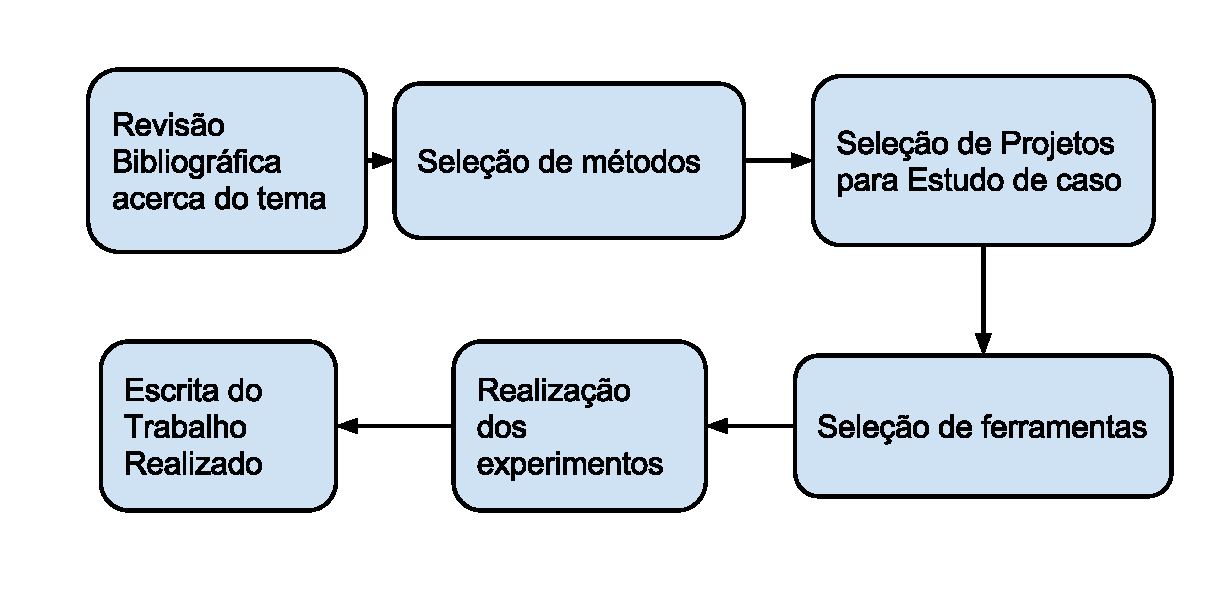
\includegraphics[keepaspectratio=true,scale=0.7]{figuras/fases_metodologia.eps}
    \caption{Fluxo de Atividades para a resolução destes trabalho}
    \label{fig:fases_metodologia}
\end{figure}


\section{Revisão Bibliográfica}

A revisão bibliográfica foi a primeira atividade realizada para a construção
 deste trabalho. Foi feito um estudo e levantamento de métodos, técnicas e
 ferramentas que podem auxiliar o desenvolvimento deste trabalho, além de
 elucidar a viabilidade da realização do mesmo. Esta revisão foi utilizada
 como referência para a  escrita da fundamentação teórica.

\section{Seleção de Métodos}

Para seleção de métodos foi realizada uma priorização dos métodos, técnicas e
 ferramentas encontradas durante a revisão bibliográfica. A priorização levou
 em conta o esforço da implementação/execução dos métodos, o tempo para a
 montagem de experimentos e o recurso computacional necessário para a criação
 destes experimentos.


Os métodos selecionados foram:

\begin{enumerate}
	\item \textit{Include Guards}, descrito na seção
 \ref{include_guards_section};
	\item \textit{Forward Declaration}, descrito na seção
 \ref{forward_declaration_section};
	\item Makefile, descrito na seção
 \ref{Makefile_section};
	\item Otimização de baixo nível;
	\item \textit{Pimpl Idiom};
	\item Compilador + \textit{Headers} pré-compilados;
	\item Ferramentas que utilizam cache de arquivos 
preprocessados (CCache, Wrap, Gold);
\end{enumerate}

\section{Seleção de Projetos}

Para a realização dos experimentos  envolvendo os métodos selecionados na
 atividade anterior foi feita uma busca de possíveis softwares livres que
 poderiam ser modificados.  As modificações seriam realizadas com o intuito
 de conseguir diferenciar o tempo de compilação de um projeto com a aplicação
 de algum dos métodos selecionados e sem  esta aplicação. Além das
 modificações, foram criados scripts para auxiliar a execução de experimentos
 que automatizassem a compilação e medissem o tempo gasto.

\subsection{Critérios de Seleção}


Para a seleção dos projetos aqui presentes foram feitos filtros de pesquisas
 na plataforma Github\footnote{\url{http://github.com}.}. Para o presente
 trabalho foram escolhidos primeiramente os 3 primeiros métodos para estudo,
 e que deveriam ser aplicados em projetos com mais de 50\% do código fonte em
 C++. Para garantir isso, foi utilizado a ferramenta sloccount para realizar
 a contagem de linhas do projeto e a percentagem de código em C++.
 A Tabela \ref{tab:projects} mostra os projetos selecionados e quais métodos
 poderiam ser aplicados.

\begin{table}[!ht]
\centering
\caption{Projetos e Métodos que podem ser aplicados}
\label{tab:projects}
\begin{tiny}
\begin{tabular}{lp{2cm}p{2cm}p{2cm}p{2cm}p{2cm}}
	\toprule
	\textbf{Projetos} & \textbf{Quantidade de linhas do projeto} & \textbf{Porcentagem em C++} &
	\textbf{Guarda de Inclusão} & \textbf{Forward declaration} & \textbf{Makefile} \\
	\midrule
	cppcheck & 136,906 & 96.02\% & Não & Não & Sim \\
	hayai & 1,668 & 83.27\% & Não & Não & Sim \\
	jsoncpp & 9,833 & 80.21\% & Não & Não & Sim \\
	libsass & 21,962 & 93.79\% & Não & Não & Sim \\
	libOauthCpp & 2,128 & 87.27\% & Não & Não & Sim \\
	Jack, the Janitor & 2,062 & 99.22\% & Não & Sim & Sim \\
	\bottomrule
\end{tabular}
\end{tiny}
\end{table}

\subsection{Projetos Selecionados}

Foram selecionados 6 projetos: cppcheck, hayai, jsoncpp, libsass,
 libOAuthcpp e Jack, the Janitor. Este projetos serão brevemente 
descritos a seguir.

\textbf{CppCheck} é uma ferramenta de código de C/C++, que detecta erros no código
 que compiladores e outras ferramentas não detectariam . Este projeto realiza
 as seguintes verificações\footnote{\url{http://cppcheck.sourceforge.net/}
 acessado em 17/06/2015.}:

\begin{itemize}
	\item índice fora dos limites do vetor;    
    \item vazamentos de memória;
    \item possíveis deferências ponteiro nulo (o que causa falhas de segmentação);
	\item existência de variáveis não inicializadas;
	\item uso inválido da STL;
	\item funções obsoletas ou com falhas de segurança; 
	\item código não utilizado ou redundante;
	\item entre outros.
\end{itemize}


\textbf{Hayai}\footnote{\url{https://github.com/nickbruun/hayai} acessado em
 17/06/2015.} é um framework para realização de benchmark em C++,utilizados
 para testes de unitários usando googletest.

\textbf{JsonCpp}\footnote{\url{https://github.com/nickbruun/hayai} acessado
 em 17/06/2015.} é uma biblioteca que permite a manipulação de arquivos .json,
 incluindo serialização e deserialização de strings. Esta pode preservar
 comentários existentes na serialização/deserialização, tornando-se um formato
 conveniente para armazenar de entradas de usuário.

\textbf{LibSass}\footnote{\url{https://github.com/sass/libsass} acessado
 em 17/06/2015.} é uma ferramenta de pré-processamento de Sass Css. Esta
 ferramenta foi originalmente criada em Ruby, no entanto a versão aqui utilizada
 é mais simples, leve, eficiente e portátil.

\textbf{LibOAuthCpp}\footnote{\url{https://github.com/sirikata/liboauthcpp}
 acessado em 17/06/2015} é uma biblioteca de C++ voltada para realizar solicitações
 de autenticação utilizando o protocolo OAuth. Ela não implementa solicitações de
 requisições em HTTP mas, no entanto, é utilizada como uma interface de suporte ao
 OAuth.

\textbf{Jack, the Janitor}\footnote{\url{https://github.com/athos-ribeiro/jtj}
 acessado em 17/06/2015;} é um jogo onde o jogador controla  a personagem Jack,
 o zelador de uma escola, que deve organizar o armazém da escola. Jack pode empurrar
 caixas para esquerda, para a direita ou saltar. O objetivo do jogo e preencher uma
 linha inteira de caixas: caso Jack seja atingido por uma caixa o jogo é finalizado
 com \textit{gameover}.

\section{Ferramentas}

As linguagens utilizadas foram C++ versão 11 e Python versão 2.7.

Para realizar a contagem do tempo foi utilizado o programa Time.
 Programa escrito por David MacKenzie e tem como objetivo indicar o tempo gasto
 por um processo em diferentes aspectos.
 O comando time tem como saída 3 tipos de valores:

\begin{itemize}
	\item User: É o tempo gasto por um processo em modo usuário;
	\item System:  É o tempo gasto por um processo em modo kernel;
	\item Real:  É o tempo total gasto na execução de um processo;
\end{itemize}

Para a coleta dos tempos foi utilizado apenas o valor Real, uma vez que este
 expressa o tempo total decorrido para a realização de um processo.

O compilador escolhido para o trabalho foi o g++. O g++ é uma melhoria do
 compilador gcc, criado pela GNU, que possui com conjunto de ferramentas
 para realiza pré-processamento, compilação, montagem e link-edição.
 No front-end,  este compilador inclui as linguagens C, C++, Objective-C,
 Fortran, Java, Ada, and Go, bem como as suas bibliotecas  (libstdc++,
 libgcj, entre outras)\footnote{\url{https://gcc.gnu.org/} acessado
 em 17/06/2015}.


Os experimentos realizados foram feitos utilizando um computador pessoal
 (notebook), com  as especificações  listadas na Tabela 
\ref{tab:especificacoes_hardware}.


\begin{table}[h]
\centering
\caption{Especificações do computador utilizado.}
\label{tab:especificacoes_hardware}
\begin{tabular}{ll}
	\toprule
	\textbf{Processador}& Intel i7 2.0Ghz \\
	\textbf{Memória RAM}         & 6GB             \\
	\textbf{Placa de Rede}       & Sim             \\
	\textbf{Sistema Operacional} & Ubuntu 15.04 \\
	\bottomrule
\end{tabular}
\end{table}


Apesar de ser um computador pessoal, uma máquina virtual utilizando Virtualbox
 foi criada para realizar um independência entre a máquina pessoal e os
 arquivos e programas pessoais, além de uma melhora  na visualização da
 diferença de tempo de compilação entre projetos\footnote{No caso de projetos menores e de compilação mais rápida, pois o 
\textit{overhead} proveniente da execução da máquina virtual torna os tempos
 absolutos de compilação maiores do que na máquina host}, independente do
 tamanho do projeto. As especificação da máquina virtual  estão listadas na
 Tabela \ref{tab:especificacoes_vm}.

\begin{table}[h]
	\centering
	\begin{tabular}{ll}
		\toprule
		\textbf{Processador} & 2 PCUs \\
		\textbf{Memória RAM} & 3 GB \\
		\textbf{Memória ROM} & 8 GB \\
		\textbf{Placa de Rede} & Sim \\
		\textbf{Sistema Operacional} & Ubuntu 14.04 \\
		\textbf{VirtualBox} & 4.3.26\_Ubuntu \\
		\bottomrule
	\end{tabular}
	\caption{Especificações máquina virtual utilizada}
	\label{tab:especificacoes_vm}
\end{table}


\section{Montagem dos experimentos e scripts}

Para a primeira etapa deste trabalho foram escolhidos 3 experimentos a
 serem aplicados.

\subsection{Experimento 1}\label{experimento_1}

Para a realização de experimentos com Inclusão de Guarda foram elaborados
 em scripts Python que criam projetos simples com a inclusão de cabeçalhos
 três vez e com diferentes tipos de inclusão, como mostrado na  Seção
 \ref{include_guards_section}.
 No apêndice geração de projetos é apresentado estes scripts.

O script cria uma pasta chamada include e, dentro dela, arquivos com o padrão
 \texttt{<NUMERO>.hpp}, que representa o nome do cabeçalho a serem incluídos no arquivo 
\texttt{main.cpp}.
 Foram criados 10 mil arquivos. Os Códigos \ref{codigo_27} e  \ref{codigo_28}
 referenciam estes modelos.



\begin{lstlisting}[language=C++,caption={Arquivo .hpp gerado pelos scripts de guardas de inclusão},
                                                   label=codigo_27]

  // <NUMERO>.hpp

  const int int<NUMERO> = <NUMERO>;

\end{lstlisting}



\begin{lstlisting}[language=C++,caption={
  Arquivo main.cpp criado pelos scripts de guardas de inclusão},
                                                          label=codigo_28]

    // main.cpp

    /* headers a serem incluidos   */

    ...


    int main(){return 0;}

\end{lstlisting}




Os scripts abordam os métodos:

\begin{itemize}
	\item guarda de Inclusão Externa;
	\item guarda de Inclusão Interna;
	\item \textit{pragma once};
	\item guarda de Inclusão Interna primeiro que \textit{pragma once};
	\item \textit{pragma once} primeiro que  Guarda de Inclusão Interna;
	\item guarda de Inclusão Externa + \textit{pragma once};
	\item redundância de Guarda de Inclusão.
\end{itemize}


A Tabela \ref{tab:modelo_guards} representa o modelo utilizado na coleta dos dados,
 contendo Guarda de Inclusão Externa(GIE), Guarda de Inclusão Interna(GGI),
 Pragma Once(PO), Guarda de Inclusão Interna Primeiro que Pragma Once(GIIPPO),
 Pragma Once Primeiro que Guarda de Inclusão Interna (POPGII),
 Guarda de Inclusão Externa e Pragma Once (GIEPO) e
 Redundância de Guarda de Inclusão(RGI).

\begin{table}[!ht]
\centering
\caption{Template de amostra de Guardas de Inclusão}
\label{tab:modelo_guards}
\begin{tiny}
\begin{tabular}{lp{1cm}p{1cm}p{1cm}p{1cm}p{1cm}p{1cm}p{1cm}p{1cm}}
\toprule
\textbf{Tipo} & \multicolumn{7}{l}{Utilização de Guarda de Inclusão} \\
\textbf{Medida} & \multicolumn{7}{l}{Tempos em segundos } \\
\textbf{Amostras} & \textbf{GIE} & \textbf{GII} & \textbf{PO} & 
\textbf{GIIPPO} & \textbf{POPGII} & \textbf{GIEPO} & \textbf{RGI} \\ \midrule
 1  &  &  &   &   &   &   &  \\ \midrule
 2  &  &  &   &   &   &   &  \\ \midrule
 3  &  &  &   &   &   &   &  \\ \midrule
 4  &  &  &   &   &   &   &  \\ \midrule
 5  &  &  &   &   &   &   &  \\ \midrule
 6  &  &  &   &   &   &   &  \\ \midrule
 7  &  &  &   &   &   &   &  \\ \midrule 
 8  &  &  &   &   &   &   &  \\ \midrule
 9  &  &  &   &   &   &   &  \\ \midrule
 10 &  &  &   &   &   &   &  \\ \midrule
 Média: & & & & &   &   &    \\ \bottomrule
\end{tabular}
\end{tiny}
\end{table}

\subsection{Experimento 2}

O segundo experimento utilizou o projeto Jack, the Janitor, no qual foi
 realizada uma refatoração dos cabeçalhos: foram incluídas forward
 declarations, os headers transferidos para o arquivo de
 implementação. Após estas modificações foi feito testes com o comando
 time e o makefile do projeto. Os valores obtidos foram armazenados no
 modelo mostrado na Tabela \ref{tab:modelo_forward_declaration}.

\begin{table}[!ht]
\centering
\caption{Template para amostras com Forward Declaration}
\label{tab:modelo_forward_declaration}
\begin{tabular}{lp{3cm}p{3cm}p{3cm}}
\toprule
\textbf{Tipo} & \multicolumn{3}{l}{Forward Declaration}\\ \midrule
\textbf{Tempo}& \multicolumn{3}{l}{Em segundos}    \\ \midrule
\textbf{Repetições} & \textbf{Sem forward Declaration(SFD)} & \textbf{Com Forward Declaration (CFD)} & \textbf{Fator de Redução (SFD/CFD)} \\ \midrule
1      &   &  &  \\ \midrule
2      &   &  &  \\ \midrule
3      &   &  &  \\ \midrule
4      &   &  &  \\ \midrule
5      &   &  &  \\ \midrule
6      &   &  &  \\ \midrule
7      &   &  &  \\ \midrule
8      &   &  &  \\ \midrule
9      &   &  &  \\ \midrule
10     &   &  &  \\ \midrule
Média  &   &  &  \\ \bottomrule
\end{tabular}
\end{table}

\subsection{Experimento 3}\label{experimento_03}

Realizar um estudo da redução do tempo de compilação utilizando o comando
 mostrado no Código \ref{codigo_29} que permite a compilação em
 múltiplas threads.


\begin{lstlisting}[language=C++,caption={
							Execução de make utilizando jobs},
                                   			 label=codigo_29]
        $ time make -j N
\end{lstlisting}

Os valores foram colocados no modelo mostrado na Tabela \ref{tab:makefile},
 com o tempo em segundos.

\begin{table}[h]
\centering
\caption{Template para amostras de Makefile}
\label{tab:makefile}
\begin{tabular}{cccccccccc}
\toprule
\textbf{Repetições} & \multicolumn{9}{c}{\textbf{Número de threads}} \\ \midrule
- & 1 & 2 & 4 & 6 & 8 & 10 & 12 & 14 & 16 \\ 
1 &   &   &   &   &   &    &    &    &  \\ 
2 &   &   &   &   &   &    &    &    &   \\ 
3 &   &   &   &   &   &    &    &    &  \\ 
4 &   &   &   &   &   &    &    &    &  \\ 
5 &   &   &   &   &   &    &    &    &  \\ 
6 &   &   &   &   &   &    &    &    &  \\ 
7 &   &   &   &   &   &    &    &    &  \\ 
8 &   &   &   &   &   &    &    &    &  \\ 
9 &   &   &   &   &   &    &    &    &  \\ 
10 &  &   &   &   &   &    &    &    & \\ \midrule
Média & & &   &   &   &    &    &    & \\ \bottomrule
\end{tabular}
\end{table}
